% !TEX root = ../thesis.tex
\chapter{Approach}
\label{ch:approach}
% **************************** Define Graphics Path **************************
\ifpdf
\graphicspath{{Chapter3/Figs/Raster/}{Chapter3/Figs/PDF/}{Chapter3/Figs/}}
\else
\graphicspath{{Chapter3/Figs/Vector/}{Chapter3/Figs/}}
\fi

\section{Introduction}
\label{sec:approachIntro}
Despite the importance of crowd monitoring in emergency management for mass gathering events, the literature review in the previous chapter has identified several gaps in the research. One of the gap is the lack of a crowd model that enables consistency and interoperability between different crowd sensing systems and applications. Another benefit of using a crowd model is to provide a standard and uniform classification of different crowds. Most state-of-the-art crowd monitoring techniques did not incorporate a crowd model to identify and distinguish different types of crowd. In other words, they lacked the capability to make distinction of different crowd types that can occur in a mass gathering event. To address this issue, our proposed approach employs one of the most widely adopted works on crowd modelling in emergency management introduced by \citet{Berlonghi1995}. Our approach also automates the classification of crowd type by capturing the emotional states of the crowd using a new source of information, that is the social media. A mapping between the crowd types and the emotions is also proposed in this approach. The emotion analysis, the crowd model and the mapping are integrated into a complete framework for a real-time crowd monitoring.

This chapter is structured as follow. Firstly, the overview of our proposed crowd monitoring framework will be introduced. Then each component in the framework will be discussed in the following sections. The chapter ends with the conclusion which will give a summarised look at the framework.

\section{An Overview of the Crowd Monitoring Framework}

The literature review in Chapter \ref{ch:litReview} shows that most of the state-of-art crowd monitoring approaches focused on using computer vision to automate the analysis of the data collected by CCTV system. The literature review also points out several limitations of the computer vision technique, such as the effect of obstacles and low lighting condition. With the rapid development of mobile computing and the increasing popularity of mobile devices, mobile sensing seems to be a potential technique to collect contextual data, from such sources as GPS receivers and accelerometers integrated in mobile devices. Context data here refers to all the information that is related to a crowd. Context data can be at raw level such as the acceleration and rotational forces generated by accelerometer built in a participant's mobile phone, or at high level such as the current activity that the user is performing inferred by activity recognition techniques.

Apart from the ``hard sensors'' where physical sensors are used, the literature review also highlights that another type of information source known as the ``soft sensor''. ``Soft sensor'' such as social media, allows monitoring the crowd and detecting the occurrence of incidents such as stampede in a crowd \citep{Ramesh2014}. The use of social media analysis for crowd monitoring has been introduced in a related work by \citet{DelirHaghighi2013}. It had the great advantage of feasibility as it only relied on the software and no additional hardware was required to be installed. In spite of this strength, our literature review shows that very limited works have been done to employ social media to support crowd monitoring in emergency management.

Secondly, the literature review shows that the actual behaviour of a crowd depends largely on the emotions of the participants \citep{Kornblum2011, jasper2011emotions}. For that reason, it is essential for a crowd monitoring approach to consider the effect of emotions in the crowd \citep{mchugh2010perceiving}. Although human emotion is an abstract concept and very difficult to measure with ``hard sensors'', it is possible to capture the emotion of a person from the verbal expressions, such as text \citep{alm2005emotions} or speech \citep{sobin1999emotion}. This is where social media further proves its advantage over the ``hard sensors''. By applying analysis on the social media, we can capture the emotions in a crowd, thus enabling the inference of the crowd's condition. For that reason, this project will propose a crowd monitoring framework that employs the emotion analysis of social media to support emergency management in mass gatherings by determining the current type of the crowd. 

Finally, the literature review also reveals another gap in the research that is the limitation of the crowd modelling employed in crowd monitoring approaches. Most existing crowd monitoring techniques did not base on any crowd model which can distinguish between different crowd types and identify the exact crowd type that is happening without the interpretation of human. By exploring broader into other disciplines, our literature review points out several notable works on crowd modelling and classification in the police literature and public safely science. Among those works, \citet{Berlonghi1995}'s work stands out as the most commonly adopted model by the emergency management bureaus worldwide. 

Our proposed crowd monitoring framework is established on the Berlonghi's model which consists of eleven different crowd types. Yet, a systematic approach to classify one crowd into those types is challenging because Berlonghi's model only describes the crowd types and there is no attribute or method defined in the existing model to make the distinction between them. Therefore, our approach will propose a mapping model that connects the emotion model with the crowd model, enabling the rule based reasoning of crowd type from emotions.

In conclusion, our proposed approach will address the gaps that are identified in the previous chapters by: 
\begin{inparaenum}[i)]
\item incorporating social media as the information source for context data;
\item capturing the emotions of a crowd by analysing the context data from soft sensors;
\item identifying the type of a crowd by applying rule based inference to the emotional states of the crowd
\end{inparaenum}. These three objectives can be integrated together in a complete process as illustrated by Figure \ref{fig:processOverview}. Social media is firstly probed to get the context data at the raw level. This raw data is then processed in an emotion analysis to extract high level context data, that is the emotional states of the crowd. Finally, these emotional states are utilized as the attributes or features to classify a crowd into specific crowd types.

\begin{figure}[htb!] 
\centering    
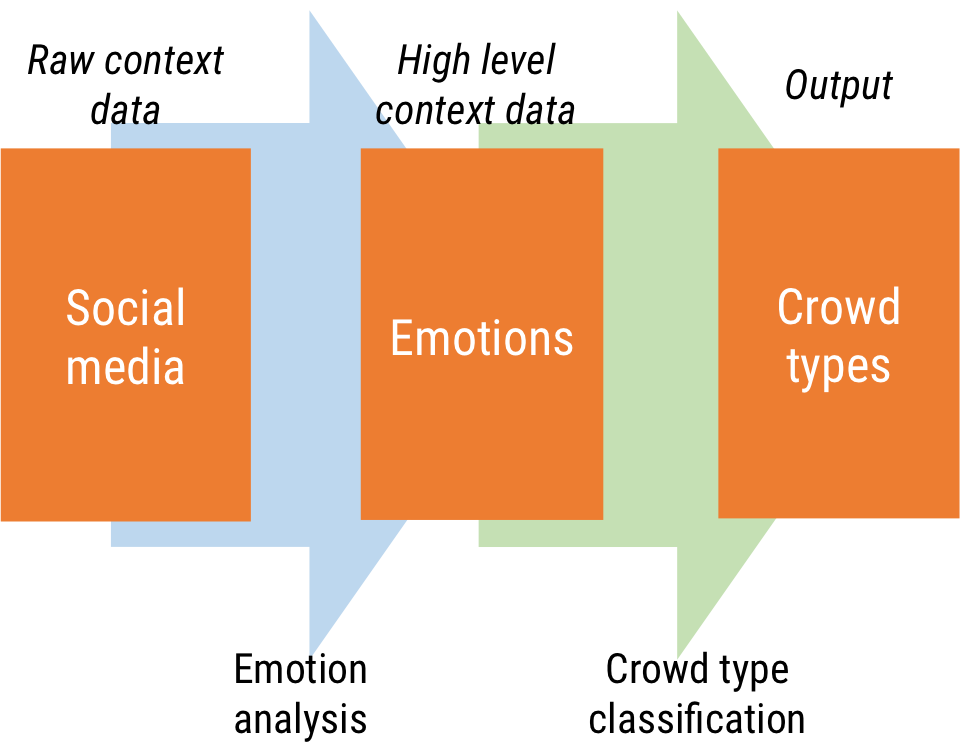
\includegraphics[width=0.5\textwidth]{ProcessOverview}
\caption{A process to identify a crowd type from social media}
\label{fig:processOverview}
\end{figure}

From the functional point of view, the process can be implemented into a framework. Figure \ref{fig:frameworkOverview} shows our framework consisting of following components:
\begin{inparaenum}[i)]
\item Context data;
\item Emotion analysis;
\item Emotion model;
\item Crowd model;
\item Emotion - Crowd type mapping model;
\item Rule based reasoning
\end{inparaenum}. Each component will be discussed further in the sections below.

\begin{figure}[htb!] 
\centering    
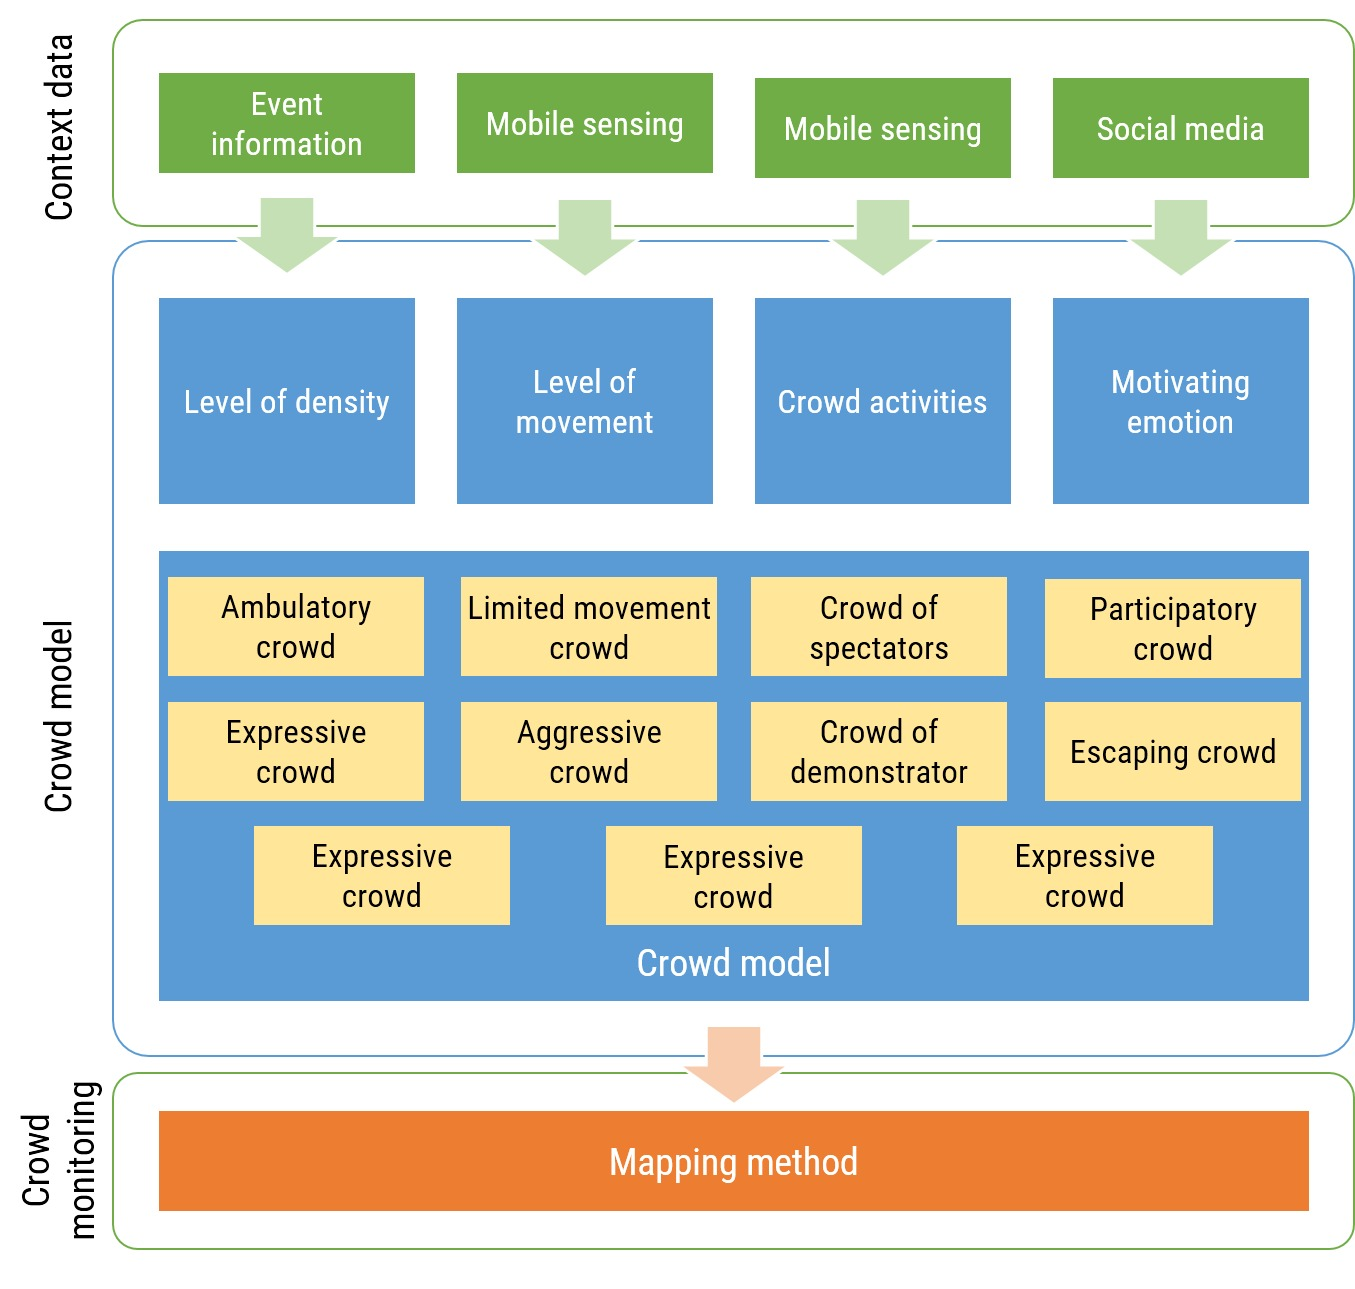
\includegraphics[width=1.0\textwidth]{FrameworkOverview}
\caption{An overview of the crowd monitoring framework using emotion analysis of social media}
\label{fig:frameworkOverview}
\end{figure}

\section{Context Data}
The first component of the framework is the Context Data component. In our proposed framework, contextual data is gathered from the social media as the information source. Social media is the generic term referring to a wide range of Internet based tools that enable a user to create and share information with each other \citep{kaplan2010users}. These tools include social network services such as Facebook and Twitter, blogs, Internet forums and channels which have marked the beginning of Web 2.0. Unlike other traditional media such as newspaper or television, the content on social media is created by the users, or also known as user-generated content \citep{kaplan2010users}. User-generated content can be in various formats such as text, image or video. Because of the fact that the content is being generated by the users themselves, social media is an effective source to obtain the knowledge about the users. In our domain and application of crowd monitoring, the kind of knowledge that is important to capture is the emotional state of the participants in the crowd. 

This research focuses on the use of social media, or Twitter in particular, as the information source for context data, because of the following reasons. Firstly, among social media, Twitter is the most commonly used in researches because of its large volume of users and its public APIs \footnote{https://dev.twitter.com/rest/public} which make the data highly accessible. The user-generated content is mostly text-based and in the form of a short message which has no more than 140 characters called tweet. Because of the length limit, a tweet is usually very simple in term of the meaning and each tweet focuses on expressing the idea of the author on one particular topic. This fact makes the semantic analysis of tweets more feasible in real-time than other content, for example, a long blog article.

A tweet might also contain information beyond the text. A significant number of tweets are geo-tagged, which means they are attached with the location information when they are posted to Twitter. This location information can be in the form of exact coordinates if the user posts the tweet from a GPS enabled mobile phone. Alternatively, this location might also be a relative location such as a point of interests or a town if the user checks in or attaches a place with the tweet.

Another useful information that might exist in a tweet is hashtags. Hashtags are created by the users, and usually are put in a tweet to refer to the topic that is mentioned in the tweet \citep{mohammad2014using}. In some mass gathering events such as the Australia Open or music festivals, there are pre-defined hashtags created for these particular events so that a user can put the hashtags into the tweet when mentioning about the events. Similarly to the geo-location, this information can also be used to filter the tweets belonging to a specific event.

Finally, using Twitter as the information source for crowd monitoring has some certain advantages. Firstly, the data can be collected in real-time, enabling the real-time monitoring which is an essential operation in emergency management because of the dynamic nature of a crowd that it can change from a calm type to an aggressive type \citep{Berlonghi1995}. Secondly, it does not require any pre-installed hardware or software on the participants' mobile devices, which increases the feasibility of the proposed framework.

\section{The Emotion Model}

According to \citet{Kornblum2011}, a crowd can be described as a form of collective behaviour of a group of people in close proximity. The other form of collective behaviour is a mass which involves people dispersed in a large area, thus does not belong to our context of emergency management in mass gathering. Both the Convergence Theory and the Emergent Norm Theory \citep{mcphail1991myth} support the idea that a crowd behaviour is formed by people with a common motivation. In our framework, emotional factor is emphasized as the common motivation of the behaviour in the crowd. Different emotions can consequently lead to different crowd behaviours. For example, according to Lofland's typology of spontaneous collective behaviours \citep{Kornblum2011}, a panic exodus from burning theatre is motivated by the \textit{fear} whereas a race riot is caused by the \textit{anger}. Therefore, an emotion model is essential to distinguish different emotions of the people in the crowd.

Human emotion is no doubt complex and confusing \citep{plutchik2001nature}. Therefore, it is difficult even to just list all emotions, not to mention modelling them. While it is often assumed among different theories of emotions that there exists a small set of basic or fundamental emotions, there is little agreement on the number of basic emotions and what emotions are in the list \citep{Ortony1990}. Based upon the theory of evolution of the biological process, \citet{plutchik2001integration} was able to identify eight basic emotions consisting of four pairs of opposite emotions: \textit{anger/fear}, \textit{joy/sadness}, \textit{trust/disgust}, \textit{anticipation/surprise}. Investigating the facial expression of human, \citet{ekman1971constants} suggested there are six basic emotions that can be universally recognised, regardless of the language. The six basic emotions are \textit{anger}, \textit{fear}, \textit{happiness}, \textit{sadness}, \textit{surprise} and \textit{disgust} as illustrated in Figure \ref{fig:emotionModel}. Ekman's model has been adopted in many researches regarding human emotions \citep{mohammad2014using, roberts2012empatweet, alm2005emotions}. 

\begin{figure}[htb!]
\centering    
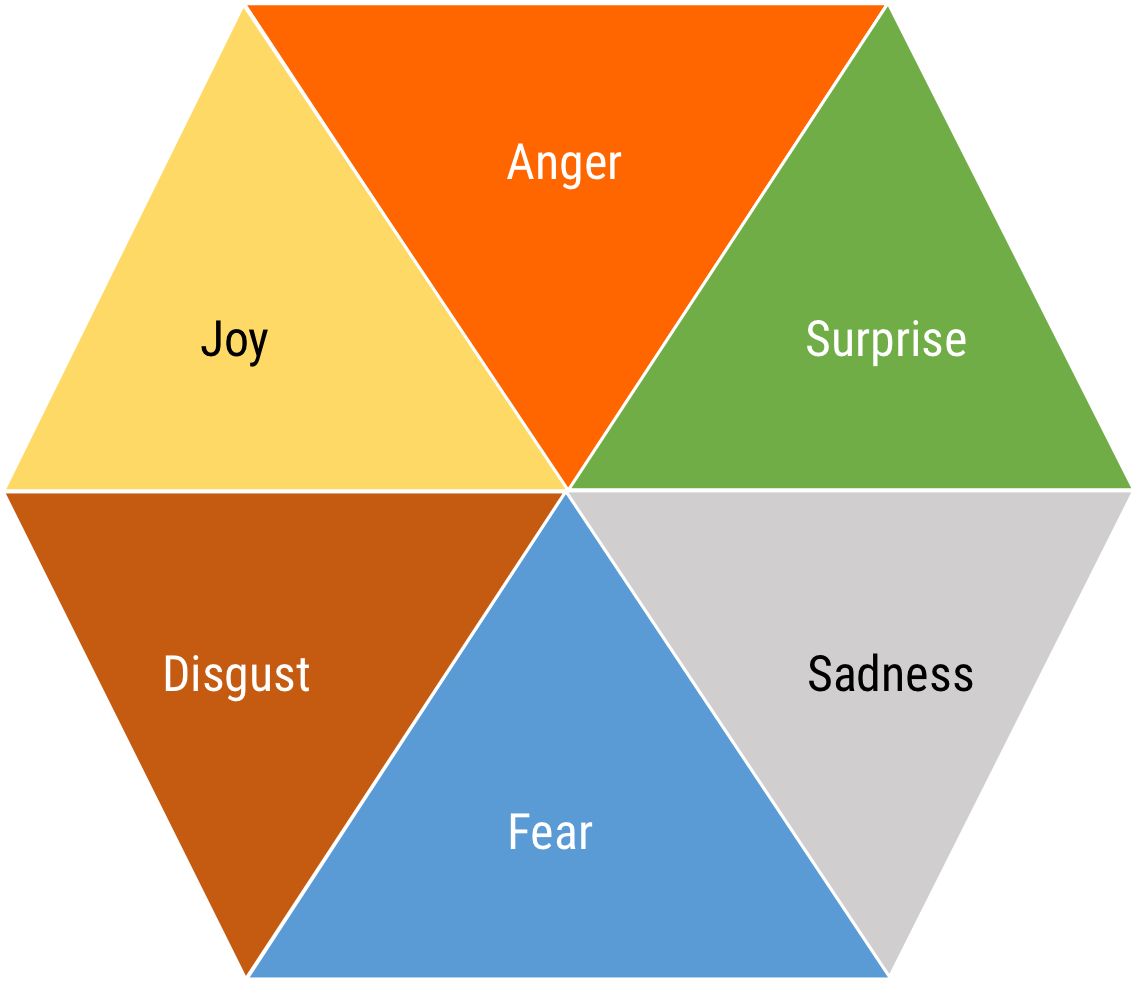
\includegraphics[width=0.75\textwidth]{EkmanModel}
\caption{Ekman's six basic emotions}
\label{fig:emotionModel}
\end{figure}

A recent research by \cite{Jack2014} has pointed out the similarity during the early signal of the facial expression between \textit{anger} and \textit{disgust}, as well as \textit{surprise} and \textit{fear}. For example, both \textit{anger} and \textit{disgust} share a wrinkled nose, while both \textit{surprise} and \textit{fear} share raised eyebrows. Based on these findings, they suggest only four basic emotions, as can be seen from Figure \ref{fig:emotionModel}.

In our proposed framework, the basic emotions are employed as the features to classify the crowd type. Because the description of the crowd types, which will be mentioned in more detail in the next section, does not specify any related emotions, it is difficult to identify which emotions associated to a particular crowd type. Using an emotion model with fewer basic emotions, each of which completely differs from the others, effectively addresses this difficulty. Therefore, the four most basic emotions consisting of \textit{anger}, \textit{fear}, \textit{happiness} and \textit{sadness} will be adopted as our emotion model in the proposed framework. Table \ref{table:emotionAnnotation} presents the four emotions and their annotations used in this research.

\begin{table}
\caption{Emotions and their annotations}
\label{table:emotionAnnotation}
\centering
\begin{tabular}{|l|l|}
\hline
\textbf{Emotion} & \textbf{Annotation)} \\ \hline \hline
Anger & \(e_1\) \\ \hline
Fear & \(e_2\) \\ \hline
Happiness & \(e_3\) \\ \hline
Sadness & \(e_4\) \\ \hline
\end{tabular}
\end{table}

\section{The Emotion Analysis of Social Media}

A recent analysis on the content on Twitter reveals that the users are using Twitter for a variety of purposes, which can be grouped in two main types: updating their statuses or sharing information \citep{java2007we}. Regardless of the content in both cases, a tweet often conveys the author's emotional status \citep{bollen2009modeling}. By capturing the emotion expressed in the text, it is possible to infer the emotional state of the author. In our framework, as can be seen from Figure \ref{fig:processOverview} a tweet can be considered as a raw context data collected from the information source whereas the emotion in the tweet is the high-level context data that is inferred and it will be used in our proposed crowd type classification. This transformation from the raw-level to the high-level context data is performed by the Emotion Analysis component. 

Regarding emotion detection from tweets, there have been several related works such as from \citet{bollen2009modeling}, EmpaTweet by \citet{roberts2012empatweet} and NRC Hashtag Emotion from \citet{mohammad2014using}. The common approach that was employed in these works is the Bag-Of-Words which only considers the occurrence of words. Our Emotion Analysis also incorporates the Bag-of-Words approach illustrated in Figure \ref{fig:bagOfWord}.

\begin{figure}[htb!] 
\centering    
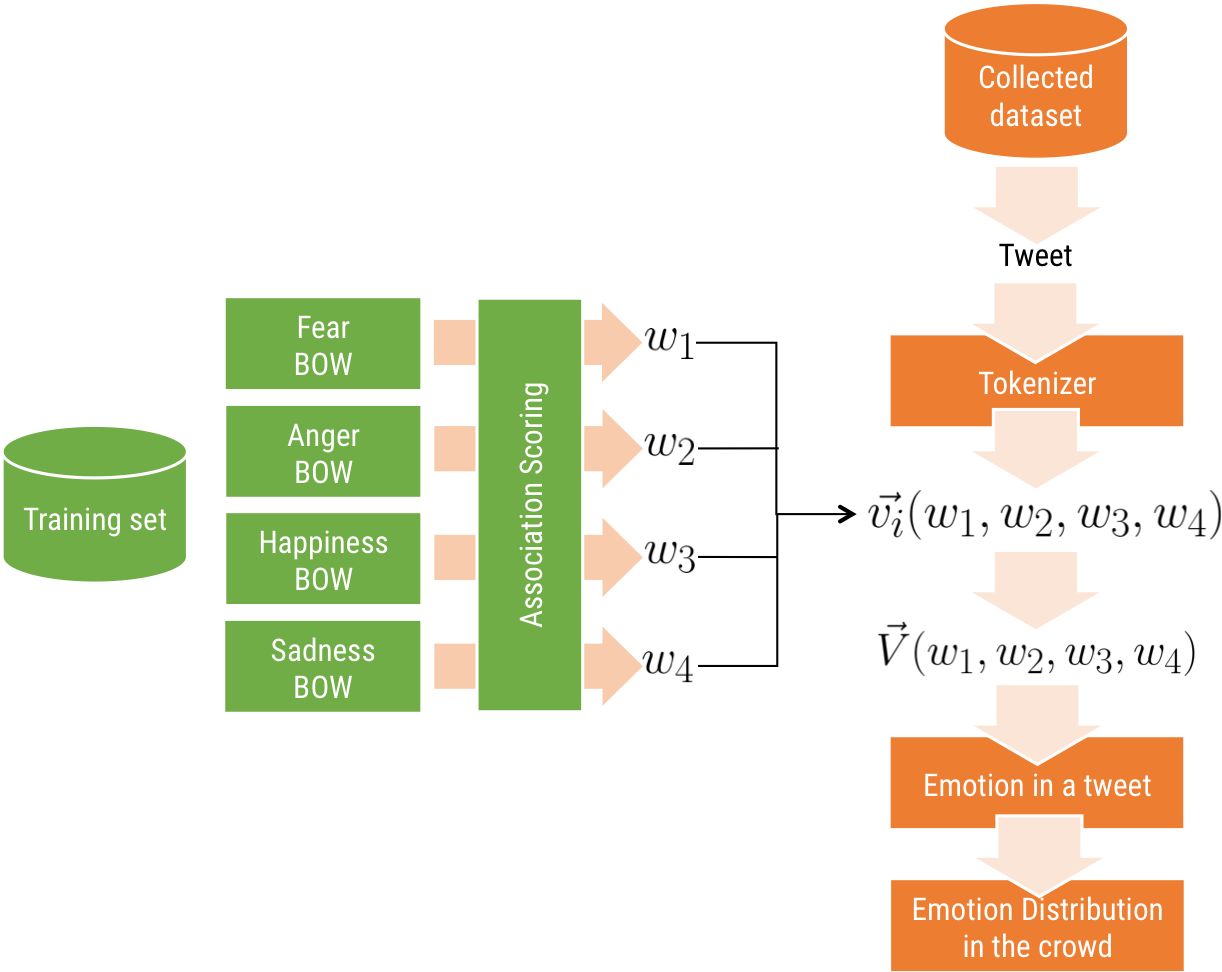
\includegraphics[width=1.0\textwidth]{BagOfWord}
\caption{An overview of the Bag-of-Words approach}
\label{fig:bagOfWord}
\end{figure}

\subsection{An Overview of the Bag-of-Words Approach}

The Bag-Of-Words approach is based on a simplified representation of a document introduced by \citet{joachims1996probabilistic}. This representation only considers at the frequency of appearance of the words in a document regardless the order of the words. In our case with Twitter, a document is a single tweet and a word is an uni-gram what builds up the tweet. The process that splits a document into a sequence of words is called tokenizer (Figure \ref{fig:tokenizer}). In our experiment which will be mentioned in Chapter \ref{ch:eval}, the Stanford Tokenizer \footnote{http://nlp.stanford.edu/software/tokenizer.shtml} is applied to tokenize a tweet into words and also to filter out unwanted text, such as URLs and emoticons.

\begin{figure}[htb!] 
\centering    
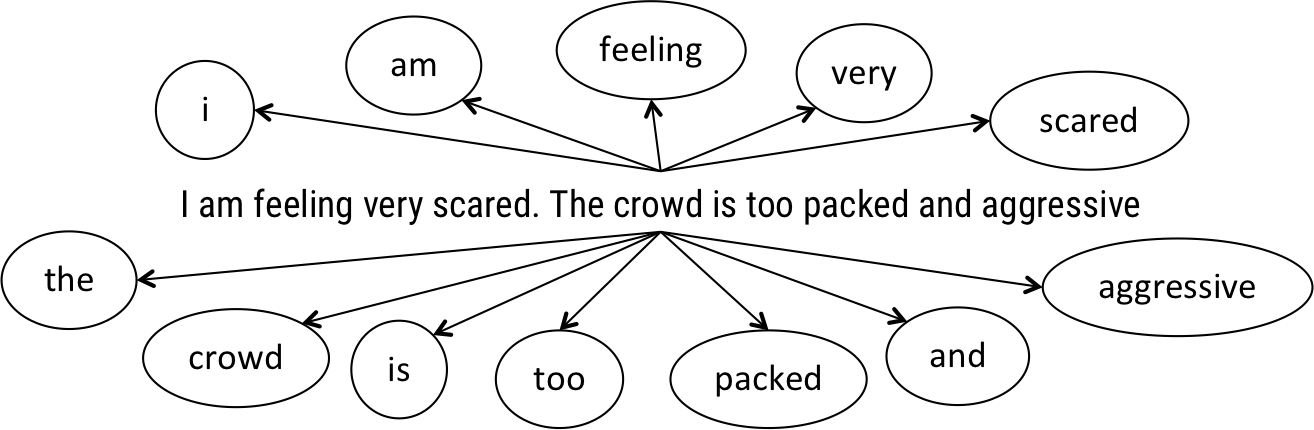
\includegraphics[width=0.5\textwidth]{Tokenizer}
\caption{An example of a tweet tokenized into words}
\label{fig:tokenizer}
\end{figure}

As mentioned earlier, most related works on emotion analysis also employed the Bag-of-Words approach. \citet{bollen2009modeling} used an extended version of the Profile of Mood States (POMS) with 765 terms from 65 original mood adjectives. These terms were used to match with the words extracted from a tweet, in order to map a tweet with the six POMS moods: \textit{tension}, \textit{depression}, \textit{anger}, \textit{vigour}, \textit{fatique} and \textit{confusion}.

The EmpaTweet by \citet{roberts2012empatweet} collected tweets on 14 selected topics that each topic was expected to evoke a particular emotion in seven emotions: \textit{anger}, \textit{disgust}, \textit{fear}, \textit{joy}, \textit{sadness}, \textit{surprise} and \textit{love}. The collected tweets formed the labelled corpus which was used to train the classifier to automatically detect the emotions from Twitter. The classification was performed by a series of Support Vector Machine (SVM) classifiers with uni-grams, bi-grams and tri-grams of words as features of a tweet.

The NRC Hashtag Emotion by \citet{mohammad2014using} was another notable work which made a good use of the hashtags as the labelled data. Tweets that were attached with these hashtags: \textit{\#anger}, \textit{\#disgust}, \textit{\#fear}, \textit{\#joy}, \textit{\#sadness} and \textit{\#surprise} and their synonyms were collected. These hashtags were considered to be the label of a tweet, which depicted the emotion in the tweet. The experiment also verified that the self-labelled hashtags were consistent and matched with the annotation by trained judges. The collected tweets constructed the NRC Hashtag Emotion Corpus. Using the corpus, \citet{mohammad2014using} computed the association of each word with Ekman's six emotions which was called the Strength of Association (SoA). This SoA score of a word can take the value from 0 for no association to infinity indicating maximum association to a specific emotion.
\begin{equation}
	0 \leq SoA < \infty
\end{equation}
The collection of words and their SoA were known as the NRC Hashtag Emotion Lexicon, which has been published and available for research purposes \footnote{http://saifmohammad.com/WebPages/lexicons.html}. 

Our Bag-of-Words approach undergoes a process illustrated in Figure \ref{fig:bagOfWord}, each step of which will be discussed in the next sections.

\subsection{The Training Set}
The training set, or labelled corpus, is a collection of tweets which are labelled with correct emotions to serve as the training data for classifiers. In this research, the NRC Hashtag Emotion Corpus by \citet{mohammad2014using} was selected as the labelled corpus because of the following advantages. Firstly, the NRC Hashtag Emotion Corpus and the EmpaTweet Corpus are were annotated with Ekman's six basic emotions, which can support our chosen four basic emotions: \textit{anger}, \textit{fear}, \textit{happiness} and \textit{sadness}. Secondly, while the EmpaTweet Corpus only collected tweets on a selected topics, the NRC Hashtag Emotion Corpus was built up from the tweets which were attached with emotional hashtags. This makes the NRC Hashtag Emotion Corpus more generic and applicable to other topics with a higher accuracy compared to the EmpaTweet which is limited to the selected topics.

\subsection{Association Scoring and the Emotional Weight Vector}
In the Association Scoring process, the association of a word with an emotion \textit{anger}, \textit{fear}, \textit{happiness} or \textit{sadness} is measured by a normalised weight. This weight represents the correlation of the appearance of the word in a tweet with the emotion extracted from that tweet. The reason for normalisation is that a weight must be comparable with the other weights of other words and other emotions. From the related works, it can be noticed that the SoA score proposed in the NRC Hashtag Emotion Lexicon by \citet{mohammad2014using} is highly suitable for this purpose. In their lexicon, the SoA of a word toward an emotion is calculated from the frequency of this word appearing in the tweets tagged with that emotion. Table \ref{table:soaOfCrowded} presented an example with the word ``crowded''.

\begin{table}[htb!]
\centering
\caption{SoA scores of the word ``crowded'' toward the eight basic emotions (Adopted from NRC Hashtag Emotion Lexicon \citep{mohammad2014using})}
\label{table:soaOfCrowded}
\begin{tabular}{|l|l|}
\hline
\textbf{Emotion} & \textbf{SoA score} \\ \hline \hline
Anger & 0.0630391396873302 \\ \hline
Fear & 0.853341316895822 \\ \hline
Joy & 0 \\ \hline
Sadness & 0 \\ \hline
Trust & 0 \\ \hline
Disgust & 0.201742824294623 \\ \hline
Anticipation & 0 \\ \hline
Surprise & 0 \\ \hline
\end{tabular}
\end{table}

In our Emotion Analysis, the SoA score from NRC Hashtag Emotion Corpus will be adopted as the normalised weight to indicate the association of a word with an emotion. The emotional status of a word is then modelled by a four dimensional vector, in which each dimension represents an emotion of the basic emotions: \textit{anger}, \textit{fear}, \textit{happiness} and \textit{sadness}. This vector is proposed as the emotional weight vector as in Formula \ref{eq:emotionalWeightVector} below.

\begin{equation}
\label{eq:emotionalWeightVector}
	\vec{v_i}(w_1, w_2, w_3, w_4)
\end{equation}
where \(v_i\) is an emotional weight vector of a word and \(w_{1,2,3,4}\) are four weights that represent its association with the four emotions: \textit{anger}, \textit{fear}, \textit{happiness} and \textit{sadness} respectively. For example with the word ``crowded'', the SoA scores are taken from the NRC Hashtag Emotion Lexicon as shown in Table \ref{table:soaOfCrowded}. The scores for \textit{anger}, \textit{fear}, \textit{joy} and \textit{sadness} are extracted and construct the emotional weight vector of ``crowded'' as in Formula \ref{eq:emotionalWeightVectorOfCrowded}.

\begin{equation}
\label{eq:emotionalWeightVectorOfCrowded}
	\vec{v_{crowded}}(0.0630391396873302, 0.853341316895822, 0, 0)
\end{equation}

\subsection{The Dominant Emotion}
The emotional status of one word can be modelled by a four dimensional emotional weight vector. A tweet can be considered as a set of words, each of which contributes to the overall emotional status of the tweet. Therefore, the emotional status of a tweet can also be represented by a four dimensional vector that is the summative of the emotional weight vectors of the elemental words (Formula \ref{eq:summativeWeightVector}).

\begin{equation}
\label{eq:summativeWeightVector}
	\vec{V} = \sum\limits_{i=1}^n \vec{v_i}(w_1, w_2, w_3, w_4)
\end{equation}
where \(\vec{V}\) is the emotional weight vector of the tweet, \(\vec{v_i}\) is a weight vector of word \(i\) and \(n\) is the total number of words in the tweet.

Although a tweet might be associated with all four emotions, the association with one specific emotion might be the most significant, which is called the dominant emotion. The summative vector \(\vec{V}\) illustrates how close the whole tweet is from each emotion. The dominant emotion of the tweet is selected as the dimension in \(\vec{V}\) which has the highest magnitude. The tweet will then be labelled with that dominating emotion. 

\subsection{Emotion Distribution, Emotion Rate and Level of Emotion}

\subsubsection{Emotion Distribution and Emotion Rate}
As illustrated by Figure \ref{fig:processOverview}, the tweets collected in the first stage of the process provides the context at the raw-level about a crowd in a mass gathering. By performing the emotion analysis, the dominant emotion in each tweet can be extracted. This emotion in fact represents the emotion of one individual in the crowd rather than the crowd as a whole. The relationship between an individual's emotion and group emotion has been discussed in several researches. \citet{barsade1998group} suggest the top-down approach that the group emotion can arise and felt by individual member, while at the same time, in a bottom-up manner the group emotion can be shaped by the compositional effects of individual emotions. This theory confirms the possibility to represent the crowd emotion as whole from the individuals' emotion.

As people with different emotional state can be in one crowd, a crowd can have multiple emotions, which can be illustrated by the emotion distribution in the crowd. In our approach, the chosen measure to represent the distribution is the emotion rate. The emotion rate \(rate(e_i)\) of an emotion \(e_i\) in a crowd in a given time period can be calculated by the following Formula \ref{eq:distributionEmotion}.
\begin{equation}
\label{eq:distributionEmotion}
	rate(e_i) = \frac{n(e_i)}{\sum\limits_{i=1}^4 n(e_i)}
\end{equation}
where \(rate(e_i)\) is the emotion rate of emotion \(e_i\) and \(n(e_i)\) is the number of tweets classified with emotion \(e_i\).

This emotion rate \(rate(e_i)\) can have any value from 0 to 1 (\(0 \geq rate(e_i) \leq 1\)), indicating the how strong the emotion \(e_i\) is during the sampling period. In order to detect the change of the emotional state in the crowd, the calculation of emotion rate is performed repetitively after an interval \(t\). The value of \(t\) has the impact on the sensitivity of the detection of the framework.

\subsubsection{Labelling the Level of Emotion}
Although the emotion distribution in a crowd is able to show the relative significance of one emotion compared to each other, it is not sufficient to tell whether a particular emotion is of abnormal behaviour or not. In this case, such linguistic labels as \textit{low} and \textit{high} are more useful to describe different levels of an emotion. While the intensity rises continuously from \textit{low} to \textit{high} level, there exists a certain point that the level of an emotion is considered to switch from \textit{low} to \textit{high} level (Figure \ref{fig:levelOfDensity}). This point is defined as threshold \(th\), which represents the expected rate of an emotion under normal behaviour. The level of an emotion can be labelled by comparing the measured emotion rate of that emotion with the threshold by Formula \ref{eq:highIntensity}.

\begin{equation}
\label{eq:highIntensity}
	rate(e_i) > th(e_i) \Rightarrow level(e_i) = high
\end{equation}
where, \(rate(e_i)\) is the emotion rate of emotion \(e_i\), and \(level(e_i)\) is the labelled level of \(e_i\).

\begin{figure}[htb!] 
\centering    
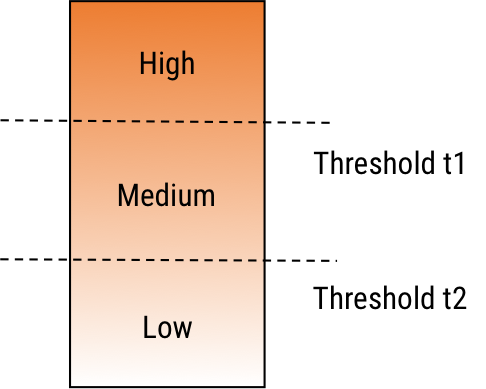
\includegraphics[width=0.3\textwidth]{LevelOfEmotion}
\caption{Level of an emotion and the threshold}
\label{fig:levelOfDensity}
\end{figure}

The threshold is important to detect the abnormal rise in an emotion, however it is application specific. Firstly, because under the normal behaviour, people tend to post an unequal number of tweets for each emotion, the thresholds can be not the same for different emotions. In fact, NRC Hashtag Emotion Corpus \citep{mohammad2014using} shows that the percentage of joyful tweet is much higher than other emotions. Secondly, because of the cultural and regional difference, the content shared on Twitter might be different across different countries and cultures \citep{Larsen2015}. 

Finally, even among the same group of users, emotional content can also vary during different time period. Analysing 509 million tweets, \citet{Golder30092011} has pointed out that people are generally less positive during winter than summer. Therefore, the value of threshold \(th\) for one emotion, such as \textit{happiness} is dependent on the region and the time of the event. In our experiment, we propose a simple approach to determine the threshold based on moving average and z-score of the emotion rate using an experimental dataset collected in a specific event.

\section{Crowd Model}

The ultimate objective of our crowd monitoring framework is to identify the type of a crowd. Therefore, a crowd model that can describe and differentiate different crowd types is required. From the emergency management point of view, the literature review highlights \citet{Berlonghi1995}'s model as one of the most significant works on crowd types. As mentioned in Chapter \ref{ch:litReview}, \citet{Berlonghi1995} has identified eleven different types of crowd in mass gathering. Each crowd type is described by the movement, participation and behaviour \citep{Zeitz2009}. Berlonghi's definition has been widely adopted as the guideline by the emergency bureaus in Australia \citep{EMA1999} and USA \citep{FEMA2005}. Eleven types of crowd are described as below.
\begin{itemize}
\item \textbf{Ambulatory crowd} - is a crowd walking in and out of a venue, to and from parking areas or walking to use restroom or concession facilities.
\item \textbf{Disability/limited movement crowd} - is a crowd of people that in some way are limited or restricted in their movement. Their level or lack of ability to walk, see, hear or speak may require more planning than is provided for all other spectators.
\item \textbf{Cohesive/spectator crowd} is a crowd watching the activities of an event or at the scene of an accident. Its primary character is the fact that people are interested in watching something specific that they came to see.
\item \textbf{Expressive/revellous crowd} - is one involved in some sort of an emotional release which can include cheering, movement in unison, celebrating, dancing, chanting or singing.
\item \textbf{Participatory crowd} - is the crowd of people involved in the actual activities of an event. Sometimes these people may be professional performers or athletes. At other times the people attending the event are participating in an actual sport, such as a marathon. Children may go up onto a stage to perform at the invitation of professional performers.
\item \textbf{Aggressive/hostile crowd} - is one that is becoming verbally aggressive towards or disregarding the instructions of ticket takers, ushers or security personnel. This crowd can get threateningly rowdy and is very open to lawlessness.
\item \textbf{Demonstrator crowd} - is one that is organised to some degree by some established leadership and whose actions may include picketing, marching, chanting or demonstrating at a particular location for a specific purpose.
\item \textbf{Escaping/trampling crowd} - is one that is attempting to escape from danger either of an actual or imagined threat to life. This includes a crowd involved in an organised evacuation procedure and a panic mob pushing and shoving with no order whatsoever.
\item \textbf{Dense/suffocating crowd} - is one in which individual physical movement is rapidly becoming less likely or impossible due to the density of the crowd. People are attempting to move,but they are either swept along with the movement of the crowd or are falling on top of each other. The results of this compression of people are fatalities and serious injuries due to suffocation.
\item \textbf{Rushing/looting crowd} - is one whose principal purpose is to obtain, acquire or steal something. This includes rushing to get the most preferred seats, autographs or actually stealing property. This very often results in fatalities, serious injuries and considerable property damage.
\item \textbf{Violent crowd} - is a crowd that is attacking, terrorising and rioting with complete disregard for laws and the rights of others.
\end{itemize}

Table \ref{table:crowdTypeAnnotation} lists eleven crowd types and their annotation used in this research. Relying only on each crowd type's description makes it difficult to identify the type of a certain crowd without human observation and judgement. Therefore, there is a need to introduce attributes or features to the existing model for a systematic approach to perform the classification of crowd type. In this proposal framework, the four basic emotions: \textit{anger}, \textit{fear}, \textit{happiness} and \textit{sadness} are introduced as the features of Berlonghi's crowd types. The next section focuses on how the mapping between each crowd type and its associated emotion is constructed.

\begin{table}
\caption{Crowd types and their annotations}
\label{table:crowdTypeAnnotation}
\centering
\begin{tabular}{|l|l|}
\hline
\textbf{Crowd type} & \textbf{Annotation} \\ \hline \hline
Ambulatory crowd & \(c_1\) \\ \hline
Disablity/Limited movement crowd & \(c_2\) \\ \hline
Cohesive/Spectator & \(c_3\) \\ \hline
Expressive/Revellous crowd & \(c_4\) \\ \hline
Participatory crowd & \(c_5\) \\ \hline
Aggressive/Hostile crowd & \(c_6\) \\ \hline
Demonstrator & \(c_7\) \\ \hline
Escaping/Trampling crowd & \(c_8\) \\ \hline
Dense/Suffocating crowd & \(c_9\) \\ \hline
Rushing/Looting crowd & \(c_{10}\) \\ \hline
Violent crowd & \(c_{11}\) \\ \hline
\end{tabular}
\end{table}

\section{Emotion - Crowd Type Mapping Model}
In the previous sections, we have discussed the possibility to detect the emotions in a crowd. In our approach, \textit{anger}, \textit{fear}, \textit{happiness} and \textit{sadness} are used as the four features of a crowd type. This section will explore further into the relationship between each crowd type and each emotion. 

Our mapping is based on several significant studies on human emotion. One of these theories is \citet{Plutchik1980}'s psychoevolutionary theory of emotion which explained emotion as a part of the evolutionary process. According to this theory, the emotional process can be modelled by a sequential model which starts with stimulus events. Based on the interpretation or cognition of these events, humans feel the emotions accordingly. The feeling state of emotion then triggers the overt behaviours or actions to achieve a desired effect. Table \ref{table:sequentialModelOfEmotion} presents the primitive sequential model of emotional process.

\begin{table}[htb!]
\caption{Sequential model of the emotional process (Adopted from \citet{plutchik2001integration})}
\label{table:sequentialModelOfEmotion}
\centering
\begin{tabular}{|p{2.5cm}|p{2.3cm}|p{2.3cm}|p{2.3cm}|p{3.5cm}|}
\hline
\textbf{Stimulus events} & \textbf{Coginition} & \textbf{Emotion} & \textbf{Behaviour} & \textbf{Effect} \\ \hline \hline
Threat & Danger & Fear & Escape & Safety \\ \hline
Obstacle & Enemy & Anger & Attack & Destroy obstacle \\ \hline
Gain of valued object & Possess & Joy & Retain or repeat & Gain resources or new genes \\ \hline
Loss of valued object & Abandonment & Sadness & Cry & Reattach with lost object \\ \hline
Member of a group & Friend & Acceptance (Trust) & Groom & Mutual support \\ \hline
Unpalatable object & Poison & Disgust & Vomit & Eject poison \\ \hline
New territory & Examine & Expectation & Map & Knowledge of territory \\ \hline
Unexpected event & What is it & Surprise & Stop & Gain time to orient \\ \hline
\end{tabular}
\end{table}

In another work, \citet{plutchik2001integration} has also summarised the relationship between emotions and their derivatives including their behaviour language, functional language and trait language. The functional language presents the pattern of adaptation to the stimulus event while the behaviour language can describe the actual actions that are derived from a specific emotion. The trait language refers to the personality that is related to that emotion. For example, \textit{fear} can trigger the escaping action for the course of protection, and it is caused by timidity. Table \ref{table:derivationOfEmotion} shows the derivation of the eight emotions including \textit{fear}, \textit{anger}, \textit{happiness} and \textit{sadness}. Although the psychoevolutionary theory is based on the basic emotions and their very primitive stimuli and derivative behaviours, it can still be applied to the modern crowd in our context. A crowd type that we can observe, can be both the stimulus events triggering the emotions or the overt behaviours triggered by the emotions. 

\begin{table}[htb!]
\caption{Emotions and their derivatives (Adopted from \citet{plutchik2001integration})}
\label{table:derivationOfEmotion}
\centering
\begin{tabular}{|p{3cm}|p{3cm}|p{3cm}|p{3cm}|}
\hline
\textbf{Emotion} & \textbf{Behaviour language} & \textbf{Functional language} & \textbf{Trait language} \\ \hline \hline
Fear & Escape & Protection & Timid \\ \hline
Anger & Attack & Destruction & Quarrelsome \\ \hline
Joy & Mate & Reproduction & Sociable \\ \hline
Sadness & Cry & Reattachment & Gloomy \\ \hline
Acceptance (Trust) & Groom & Incorporation & Trusting \\ \hline
Disgust & Vomit & Rejection & Hostile \\ \hline
Expectation & Map & Exploration & Demanding \\ \hline
Surprise & Stop & Orientation & Indecisive \\ \hline
\end{tabular}
\end{table}

Regarding the emotional language, another notable work that plays an important role in our construction of the mapping is from \citet{russell1980circumplex}. In this study, 28 emotional words are placed into a two dimensional space based on their degree of arousal and pleasure (see Figure \ref{fig:emotionSpace}). These affective words include \textit{angry}, \textit{afraid}, \textit{happy} and \textit{sad} which are used to refer the four basic emotions: \textit{anger}, \textit{fear}, \textit{happiness} and \textit{sadness} respectively. From this map, the relative position of a word from the four basic emotions can be observed.

\begin{figure}[htb!] 
\centering    
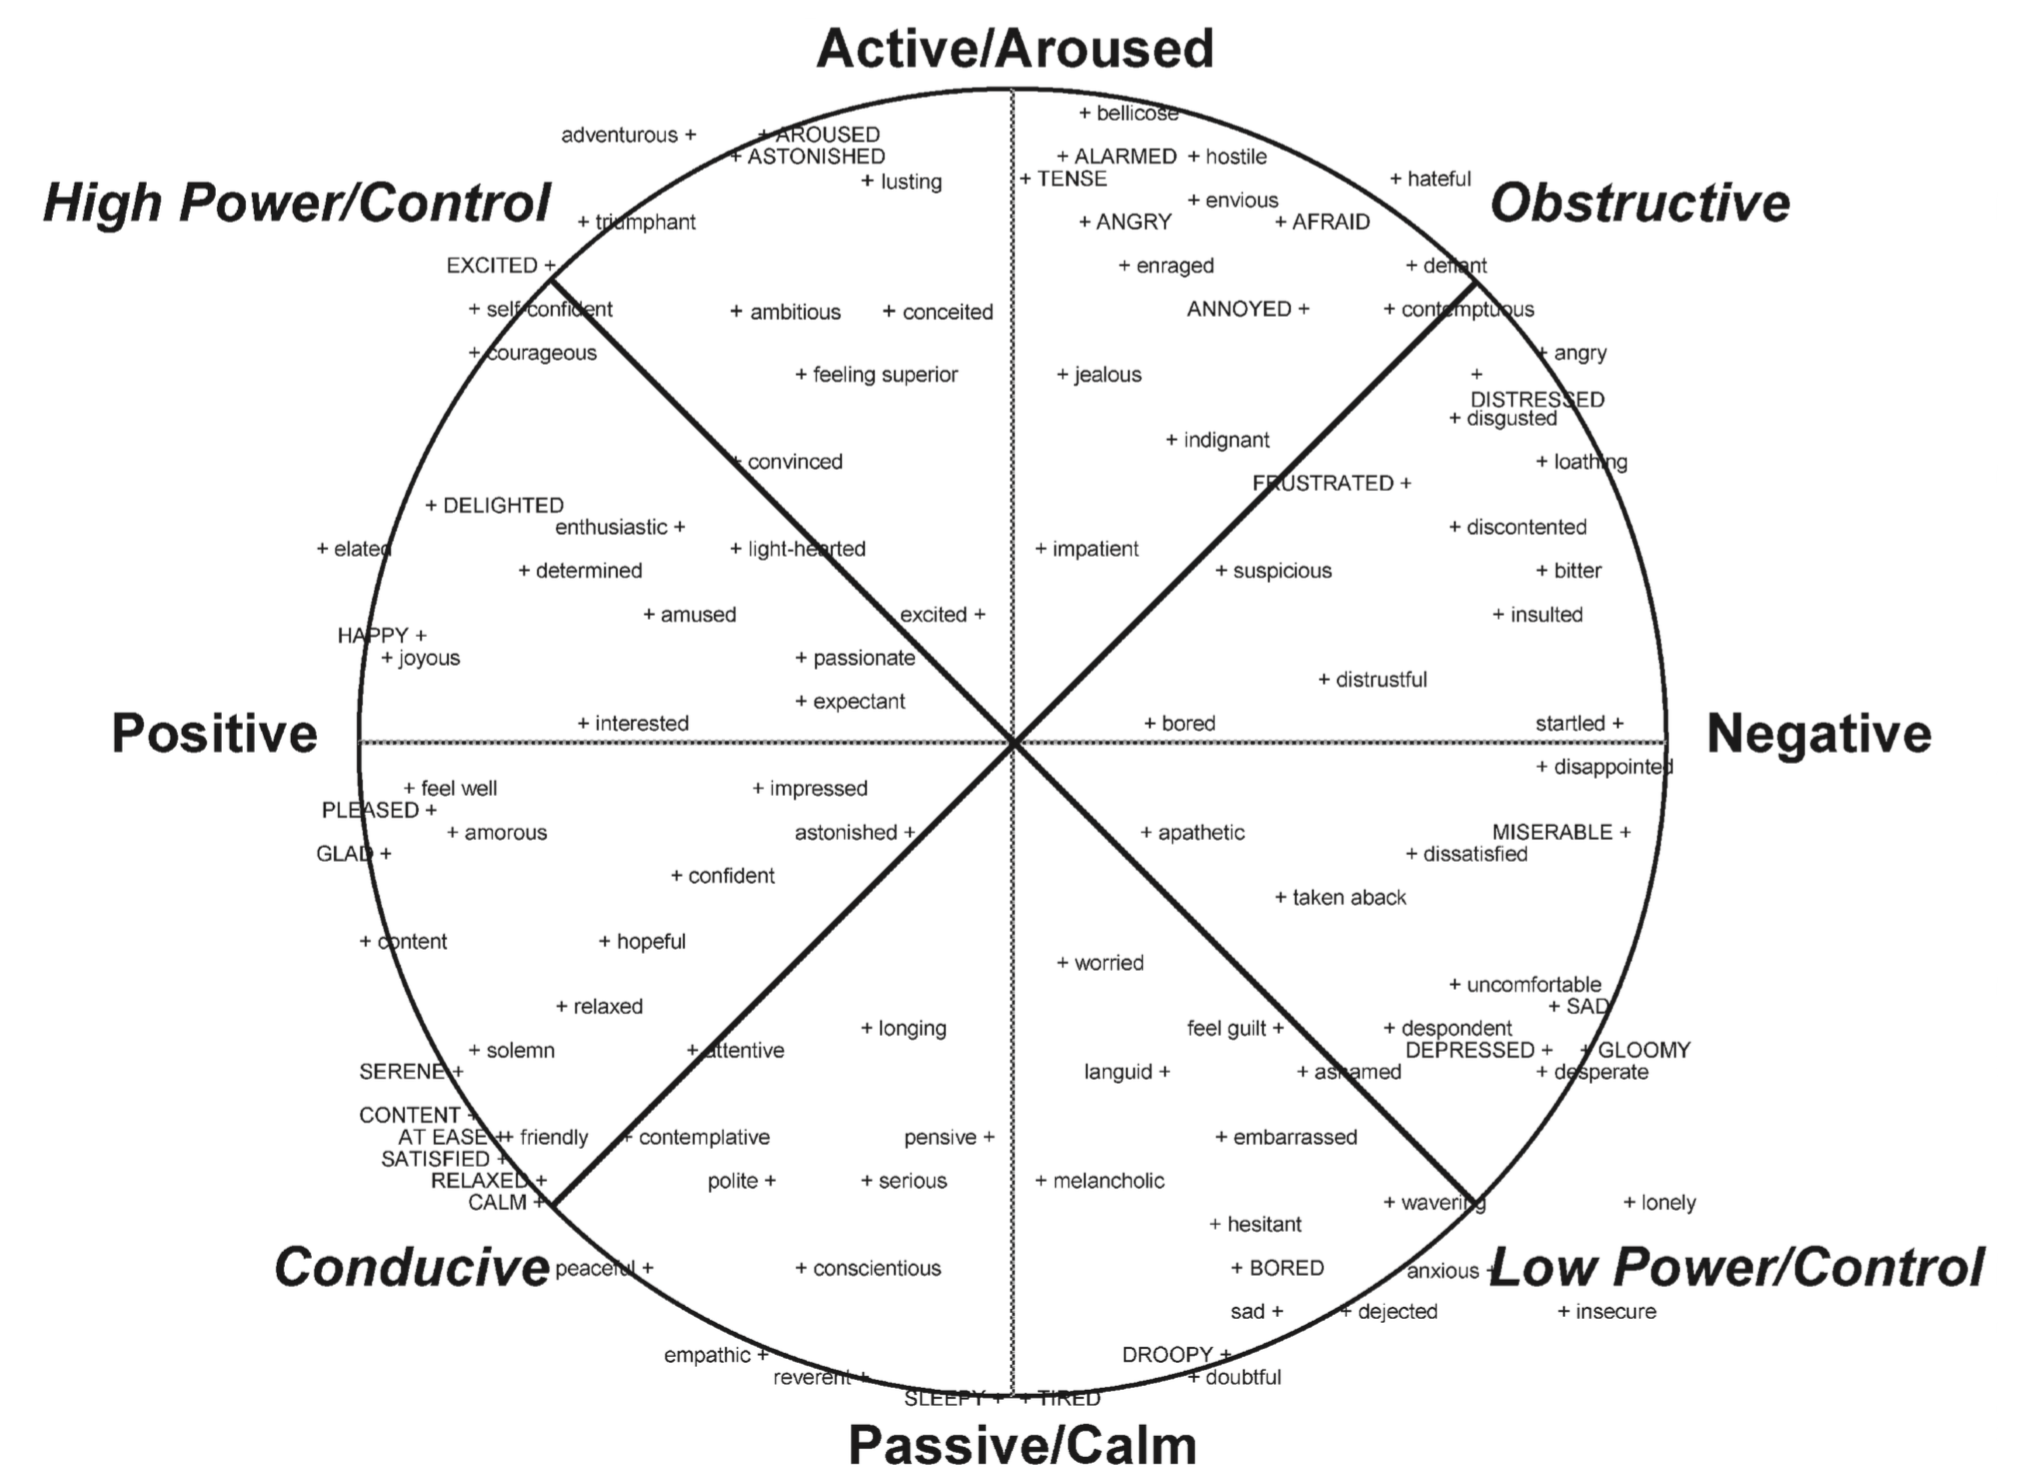
\includegraphics[width=1.0\textwidth]{EmotionSpace}
\caption{Russell's two dimensional map of emotion space (Adopted from \citet{scherer2005emotions})}
\label{fig:emotionSpace}
\end{figure}

In order to construct the emotion - crowd type mapping, a comprehensive understanding of the behaviour of each crowd type is needed. The description of each crowd type by \citet{Berlonghi1995} is analysed together with the definition of similar crowd types defined by other scholars. The behaviour language and trait language from those descriptions are extracted and referenced to the four emotions: \textit{anger}, \textit{fear}, \textit{happiness} and \textit{sadness}. The objective of this process is to identify the possible dominant emotions in each crowd type. 

\begin{itemize}
\item \textbf{Ambulatory crowd} - is characterised by the action walking and the calmness \citep{Zeitz2009}. According to \citet{russell1980circumplex}'s emotion space, \textit{calm} is located in a completely opposite region with \textit{angry} and \textit{afraid}. Although both \textit{calm} and \textit{sad} have negative level of arousal, the former has a positive degree of pleasure while the latter does not. Therefore, none of the four emotions are dominating in this crowd type.

\item \textbf{Disablity/Limited movement crowd} - is described by the immobility of the crowd. Similarly to the ambulatory crowd, this characteristic does not suggest any significant emotion. Hence, no emotion is considered to be the dominant emotion in this crowd type.

\item \textbf{Cohesive/Spectator} - is described by the activity watching a specific event and the fact that people have the interest in watching the event. Similarly, they do not signal the dominant occurrence of any emotion.

\item \textbf{Expressive/Revellous crowd} - is characterised by the emotional release. According to the Webster's Revised Unabridged Dictionary \footnote{http://www.thefreedictionary.com/revelous}, the word \textit{revelous} originates from ``revel'' which means ``to take great pleasure or delight'' \footnote{http://www.thefreedictionary.com/reveling}. \textit{Delighted} lies in a high level of arousal with a positive pleasure in the \citet{russell1980circumplex}'s emotion space (Figure \ref{fig:emotionSpace}), which is close to \textit{happy}. Therefore, it can be inferred that this crowd type has a high level of \textit{happiness} as the dominant emotion.

\item \textbf{Participatory crowd} - is described by the action participating in a specific event. Although, the description does not suggest any clue on the emotional state of the participants, one example for a participatory crowd is people taking part in an actual sport event. Regarding sport psychology, studies show that sensation seeking and arousal seeking motivate the participations in sports, especially risk involved sports \citep{rowland1986sensation}. This indicates a high level of arousal that can be observed from a participatory crowd, thus suggesting \textit{happiness} as the dominating emotion as well.

\item \textbf{Aggressive/Hostile crowd} - is described by the verbal aggressiveness and disregard for instruction. \textit{Aggressiveness} is aroused by \textit{anger}.

\item \textbf{Demonstrator} - includes such actions as picketing, marching, protesting. According to Lofland's typology of spontaneous collective behaviours \citep{Kornblum2011}, such crowds are classified into \textit{hostile} crowd aroused by \textit{anger}.

\item \textbf{Escaping/Trampling crowd} - is described by the escaping action from a danger or a threat. This \textit{escaping} behaviour is triggered by \textit{fear} according to Plutchik's evolutionary theory. Loftland's typology also classifies such crowd under the fearful crowd \cite{Kornblum2011}. Hence, the dominating emotion can be identified in this crowd type is a high intensity of \textit{fear}.

\item \textbf{Dense/Suffocating crowd} - is characterised by the extremely high density and inability of movement in the crowd. Recent research on brain claims that suffocation might cause \textit{fear} as the experiments with mice shows that inhaled carbon dioxide reduces brain pH and evokes the \textit{fear} behaviour \citep{ziemann2009amygdala}.

\item \textbf{Rushing/Looting crowd} - is described by the desire to acquire something. Studying the looting behaviour in London riot in 2011, \citet{ray2014shame} suggests the shame theory of violence which might has relevance in accounting for the violent disturbance. \textit{Shame} falls into the region with low arousal and negative pleasure together with the basic emotion \textit{sad}, which indicates the closeness of the two affective words. On the other hand, violence is aroused by \textit{anger}, hence a mixture of \textit{anger} and \textit{sadness} can be considered the dominating emotions in a looting crowd.

\item \textbf{Violent crowd} - is described by the attacking, terrorising and rioting action with the complete disregard for laws and other people. Attacking is a typical behaviour triggered by \textit{anger}. This crowd type has a high level of \textit{anger}.
\end{itemize}

As we can notice from the above analysis, five distinct groups of crowd types can be identified by their similarity in term motivating emotions (Table \ref{table:crowdTypeGroup}). Although it might be challenging to distinguish different crowd types in the same group using the emotional states as the criteria, it is possible to extend the framework and incorporate additional information sources and analysis techniques to provide additional contextual information. This information includes low level and high level context data that can improve the classification of crowd types. For example, using activity recognition over the data collected from accelerometers built on participants' mobile devices, the crowd movement can be inferred and used as an additional crowd feature in crowd type classification. 

However, obtaining data from the sensors in participants' mobile phones requires installing software on those devices, which might cause the hesitance to share information or raise privacy concern. Our proposed mapping only considers on the social media analysis, which is more feasible in favour of deployment.

\begin{itemize}
\item The \textbf{first group} consists of ambulatory, disability/limited movement and cohesive/spectator crowd, which is not associated with any emotion. From the emergency management point of view, those three types do not pose potential danger. Therefore, in our crowd monitoring framework, the three crowd types will be grouped and monitored as a same type. As mentioned earlier, if data from accelerometer built into the participants' mobile devices can be acquired, the activities of participants in the crowd can be inferred using an activity recognition technique. In term of the type of activity, an ambulatory crowd involves mostly walking, while a crowd of spectators or limited movement crowd will be more stationary which can be identified by sitting or standing activity.

\item The \textbf{second group} is characterised by \textit{happiness}. Expressive/revellous and participatory crowd belong to this group. To further distinguish between these two crowd types, using accelerometer and activity recognition to infer the activities of the participants could provide a better understanding of a crowd type. If the activities involve a high level of movement such as running and walking, the crowd can be identified as a participatory crowd.

\item The \textbf{third group} is aroused by \textit{anger} and includes demonstrator, aggressive/hostile and violent crowd with the increasing level of anger. Activity recognition can also be used to give additional knowledge. A violent crowd involves activities that have a higher level of motion such as running and walking, while a demonstrator crowd might have a slower pace of movement.

\item The \textbf{fourth group} is motivated by \textit{fear} consisting of escaping/trampling and dense/suffocating crowd. Because a dense/suffocating crowd is characterised by the high density and the inability to move, this crowd type can be identified with most people standing by activity recognition.

\item The \textbf{fifth group} is rushing/looting crowd which has both \textit{anger} and \textit{sadness} as the dominant emotions.
\end{itemize}

\begin{table}
\centering
\caption{Groups of crowd types based on common motivating emotion}
\label{table:crowdTypeGroup}
\begin{tabular}{|p{1.5cm}|p{9cm}|p{3.5cm}|}

\hline
\textbf{Group} & \textbf{Crowd types} & \textbf{Motivating emotion} \\ \hline \hline
Group 1 & Ambulatory, Limited movement/Disability, Spectator & none \\ \hline
Group 2 & Expressive/Cohesive, Participatory crowd & \textit{happiness} \\ \hline
Group 3 & Demonstrator, Aggressive crowd, Violent crowd & \textit{anger} \\ \hline
Group 4 & Escaping crowd, Dense/Suffocating crowd & \textit{fear} \\ \hline
Group 5 & Rushing/Looting crowd & \textit{anger} and \textit{sadness} \\ \hline
\end{tabular}
\end{table}

\section{Rule Based Reasoning}

The Rule Repository contains the rules to identify a crowd type or a group of crowd type from the inferred emotional state of the crowd. 

Let \(c\) be the crowd type \(c \in \{c_1, c_2, c_3, c_4, c_5, c_6, c_7, c_8, c_9, c_{10}, c_{11}\}\) as annotated in Table \ref{table:crowdTypeAnnotation}. Let \(e\) be the emotion \(e \in \{e_1, e_2, e_3, e_4\}\) as annotated in Table \ref{table:emotionAnnotation}. The \(level(e_i)\) is the level of intensity of emotion \(e_i\). The rules are defined in following formulas.

\begin{equation}
\label{eq:rule1}
\begin{split}
	(level(e_1) \neq high) \land (level(e_2) \neq high) \land (level(e_3) \neq high) \land (level(e_4) \neq high) \\
	\Rightarrow (c = c_1) \lor (c = c_2) \lor (c = c_3)
\end{split}
\end{equation}

\begin{equation}
\label{eq:rule2}
	level(e_3) = high \Rightarrow (c = c_4) \lor (c = c_5)
\end{equation}

\begin{equation}
\label{eq:rule3}
	level(e_1) = high \Rightarrow (c = c_6) \lor (c = c_7) \lor (c = c_{11})
\end{equation}

\begin{equation}
\label{eq:rule4}
	level(e_2) = high \Rightarrow (c = c_1) \lor (c = c_8) \lor (c = c_9)
\end{equation}

\begin{equation}
\label{eq:rule5}
	(level(e_1) = high) \land (level(e_4) = high) \Rightarrow (c = c_{10})
\end{equation}

The Rule Based Reasoning applies the rules defined in the Rule Repository. The input is the level of emotions obtained from the Emotion Analysis. The output is a specific crowd type or a group of similar crowd types in term of motivating emotion. It is notable that each rule is processed independently, which allows multiple crowd types to exist in one specific event.

\section{Conclusion}
This chapter has proposed a Crowd Monitoring Framework based on the Emotion Analysis of Social Media. In our proposed framework, Twitter provides the low level context data about a mass gathering event. The Emotion Analysis employs the Bag-of-Words approach and a summative vector method to detect the dominating emotion from the tweet, which is either \textit{anger}, \textit{fear}, \textit{happiness} or \textit{sadness}. From the distribution of those emotions in the crowd, the level of each emotion is labelled as \textit{low} or \textit{high}. A mapping model from emotion to crowd type has also been introduced to map the crowd emotions to the crowd types or group of crowd types. The Rule Based Reasoning converts the mapping model into rules and applies the rules to perform crowd type classification. The next chapter will describe the implementation and evaluation of the proposed framework using a case study.